\textbf{UI Design:}
\newline
Ein gutes Beispiel für ein gelungenes UI Design sind die Switches von IOS. Es ist am ersten Blick klar, was der Zustand des Switches ist, also ob er ein- oder ausgeschaltet ist. Dieses Element ist bereits bei einem Großteil der Benutzer:innen bekannt und hat sich in dieser Art gut etabliert.

\begin{figure}[h!]
    \centering
    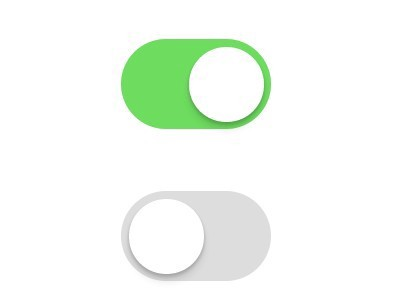
\includegraphics[width=0.5\textwidth]{pics/ui-example.png}
    \caption{UI Beispiel}
    \cite{frontend_ui_ux}
    \label{fig:mesh1}
\end{figure}
\newpage
\textbf{UX Design}
\newline
Ein Beispiel für ein gelungenes UX Design ist die Suchfunktion von Google. Wenn ein Text eingegeben wird erscheinen in einem Dropdown zahlreiche passende Suchvorschläge. Diese Funktion ist im Allgemeinen nichts besonderes für die meisten, da es durch die Verwendung bereits selbstverständlich wurde. Dies ist jedoch ein perfektes Beispiel für ein gutes UX-Design.

\begin{figure}[h!]
    \centering
    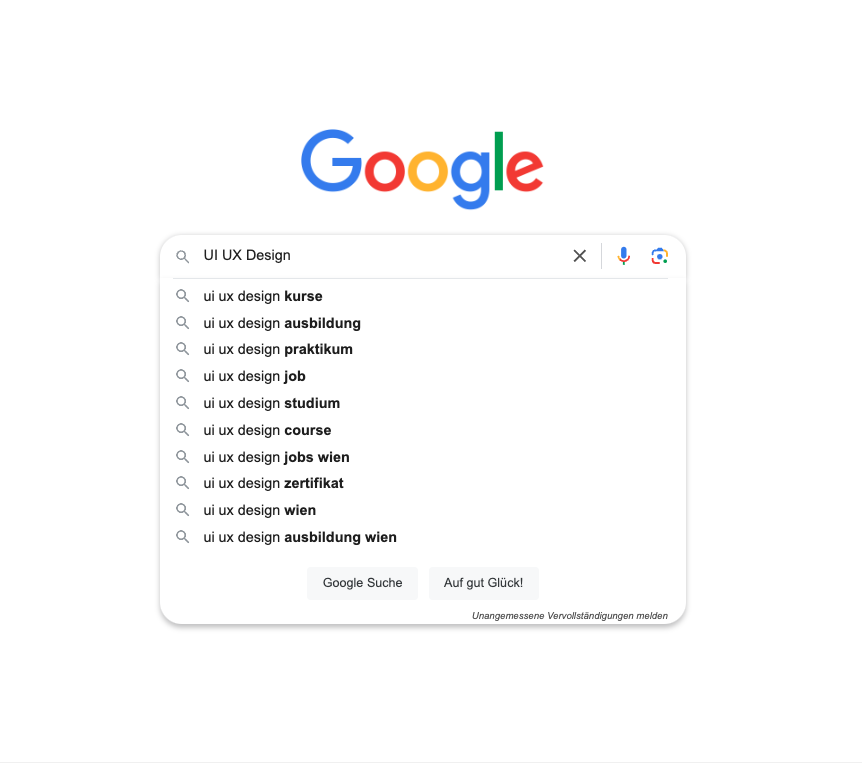
\includegraphics[width=1\textwidth]{pics/ux-example.png}
    \caption{UX Beispiel}
    \cite{frontend_ui_ux}
    \label{fig:mesh1}
\end{figure}

\cite{frontend_ui_ux}